\chapter{Progress in Project}

\section{Implementation}

The Farming Intelligence AI system has been implemented as an integrated agricultural decision-support platform combining IoT-based soil monitoring, machine learning, agricultural advisory, explainable AI, market intelligence, and a retrieval-augmented AI assistant. The implementation connects the different modules so that the collected farm data can be processed and presented to the farmer through a unified web-based interface.

\subsection{Module Split-up}

\subsubsection{Data Acquisition and Pre-processing Module}

The data acquisition module collects the agricultural parameters required by the system. The implemented IoT setup uses an ESP32 connected to a 7-in-1 soil sensor for obtaining soil moisture, temperature, pH, electrical conductivity, nitrogen, phosphorus and potassium values. Weather information is obtained through the weather service to provide additional environmental parameters such as temperature, humidity and rainfall. The system also supports manual entry of soil values when required. The collected values are validated and processed before being passed to the other modules. This ensures that the input data is suitable for crop recommendation and agricultural advisory.

\subsubsection{Crop Recommendation Module}

The crop recommendation module is responsible for identifying suitable crops based on the available soil and environmental conditions. The implemented model uses nitrogen, phosphorus, potassium, temperature, humidity, pH and rainfall as input parameters. The machine learning model analyzes these values and generates suitable crop recommendations. Multiple suitable crops can be presented to the farmer, allowing comparison instead of limiting the result to a single crop. The recommendation results are also used by other modules such as fertilizer advisory, irrigation guidance, explainable AI and market intelligence.

\subsubsection{Fertilizer and Irrigation Advisory Module}

The fertilizer and irrigation advisory module provides practical recommendations based on the selected crop and the available farm conditions. The system compares the soil nutrient values with the requirements of the recommended crop and identifies nutrient-related requirements. Irrigation guidance is generated by considering soil moisture along with available rainfall and weather information. The module also considers the pH condition of the soil and provides suitable corrective guidance when necessary. This converts the crop recommendation into actionable farming advice.

\subsubsection{Explainable AI Module}

The Explainable AI module is implemented to make the machine learning recommendations easier to understand. The system uses SHAP and LIME techniques to analyze the contribution of input features to the prediction. The important factors affecting the predicted crop are presented in an understandable manner. Instead of providing only a prediction, the system explains why the crop was recommended based on the given soil and environmental conditions. This improves the transparency and interpretability of the recommendation process.

\subsubsection{Market Intelligence and Price Forecasting Module}

The market intelligence module provides information that helps farmers evaluate the economic potential of recommended crops. The system uses available market data to analyze price trends and estimate future prices. Expected yield, forecasted price and cultivation cost are considered to estimate the potential profitability of a crop. The resulting information is presented to the farmer along with market-related indicators to support better decision-making. This module allows the farmer to consider both the agricultural suitability of a crop and its potential economic return.

\subsubsection{Retrieval-Augmented Generation Assistant}

The RAG-based agricultural assistant provides an interactive way for users to obtain agricultural information. Relevant agricultural documents are processed and stored in a searchable knowledge base. When the user submits a question, the system retrieves relevant information from the knowledge base and provides it as context to the AI model. The assistant then generates a response based on the retrieved information. This approach helps the system provide more relevant and document-based agricultural guidance instead of relying only on general language-model knowledge. The implemented workflow includes document processing, chunking, embeddings, vector storage, retrieval and answer generation.

\subsubsection{Multilingual Support Module}

The multilingual support module is implemented to make the system accessible to users who prefer different languages. The interface can display important system information according to the selected language, while the agricultural assistant can provide responses in the user's preferred language. This improves the usability of the system for farmers who may not be comfortable using English for agricultural queries. The multilingual functionality is integrated with the main dashboard and AI assistant.

\subsubsection{Alerts and Notifications Module}

The alerts and notifications module monitors important farm conditions and generates alerts when predefined conditions are detected. Conditions such as low soil moisture, significant weather changes and sensor-related problems can be used to generate notifications. The alerts help farmers identify conditions that may require immediate attention. The information can be displayed through the dashboard so that the user can respond to changing farm conditions in a timely manner.

\subsubsection{User and Admin Management Module}

The user and admin management module provides controlled access to the application. Users can manage their farm-related information and access the available agricultural services. The administrator has additional privileges for managing system-level information and resources. Authentication and access control are used to separate user and administrative functionalities. This provides a structured environment for managing the application while protecting user-specific farm information.

\subsection{Tools and Techniques}

\subsubsection{Frontend Development}

The frontend of the system is developed using React with TypeScript and TSX. HTML5 is used for the basic web structure, while CSS3 and Tailwind CSS are used for styling and responsive interface design. The frontend provides the dashboard through which users can access farm information, crop recommendations, advisory results, market intelligence, IoT readings, XAI explanations and the agricultural AI assistant.

\subsubsection{Backend Development}

The backend is implemented using TypeScript and JavaScript with Node.js. The backend manages application logic, data processing, API communication and interaction between the different modules. It also supports communication between the frontend and external services required by the system.

\subsubsection{Machine Learning and Explainable AI}

The crop recommendation system uses machine learning to process soil and environmental parameters and generate crop predictions. SHAP and LIME are incorporated to provide explanations for the generated recommendations. The machine learning workflow includes data preparation, model training, prediction and interpretation.

\subsubsection{Database and Cloud Services}

Firebase Firestore is used as the cloud database for storing and managing application-related data. Firebase authentication and security rules are used to control access to the system. The cloud-based architecture allows the application and its data services to be accessed through the web platform.

\subsubsection{IoT and Sensor Communication}

The IoT component uses an ESP32 connected to a 7-in-1 soil sensor through Modbus RTU communication. The sensor provides soil parameters including N, P, K, pH, moisture, temperature and electrical conductivity. The ESP32 reads the sensor values and transfers the collected data to the application for monitoring and further processing.

\subsubsection{AI and RAG Technologies}

The AI assistant uses a retrieval-augmented generation approach in which agricultural knowledge is retrieved from a prepared knowledge base before generating a response. Documents are divided into smaller sections, converted into embeddings and stored in a vector database. Relevant information is retrieved according to the user's question and supplied to the language model for generating the final response.

\begin{figure}[htbp]
    \centering
    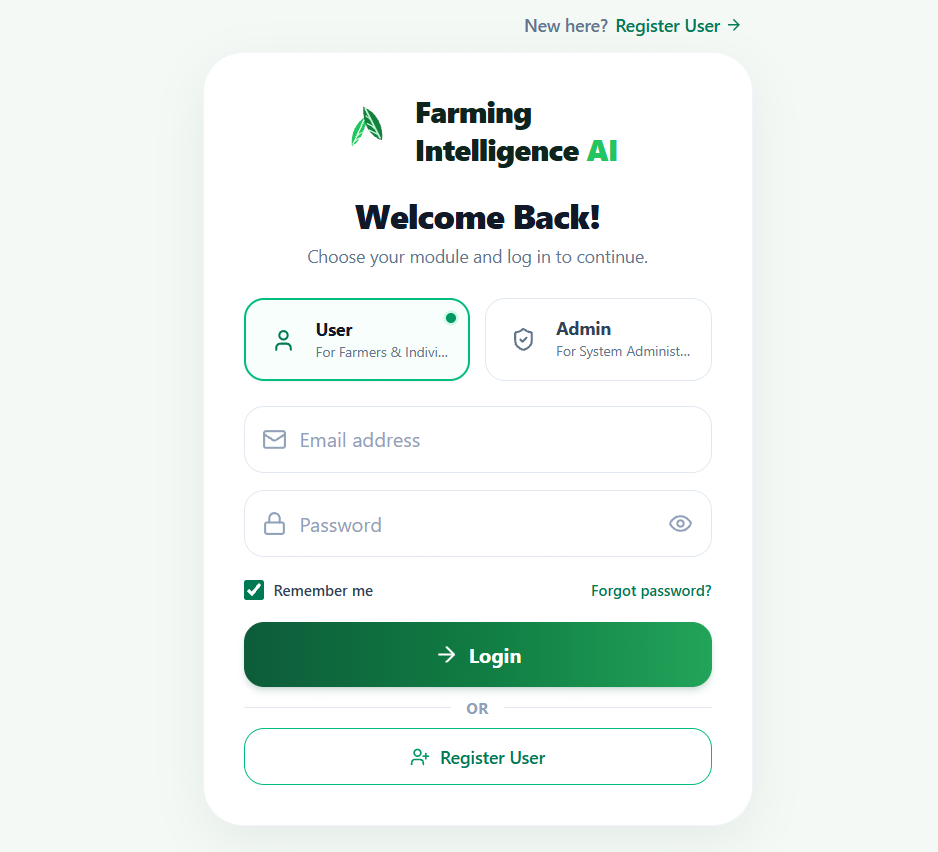
\includegraphics[width=0.6\linewidth]{img/login_page.png}
    \caption{Login Page}
    \label{fig:login_page}
\end{figure}

\begin{figure}[htbp]
    \centering
    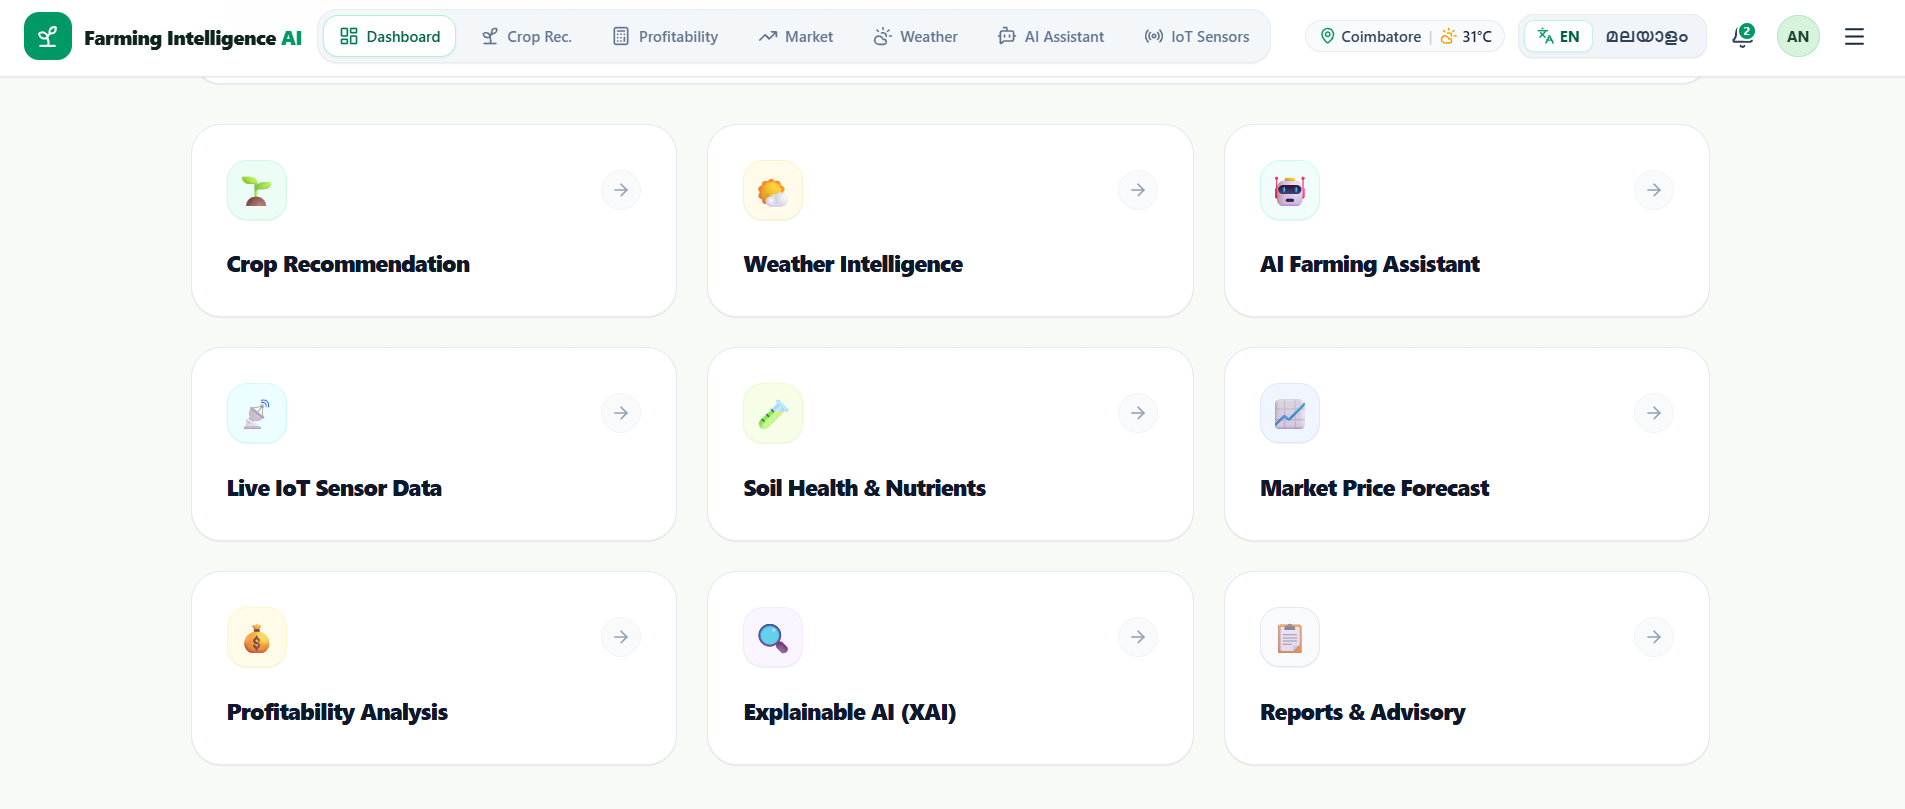
\includegraphics[width=0.8\linewidth]{img/dashboard.png}
    \caption{Farming Intelligence AI Dashboard}
    \label{fig:dashboard}
\end{figure}

\begin{figure}[htbp]
    \centering
    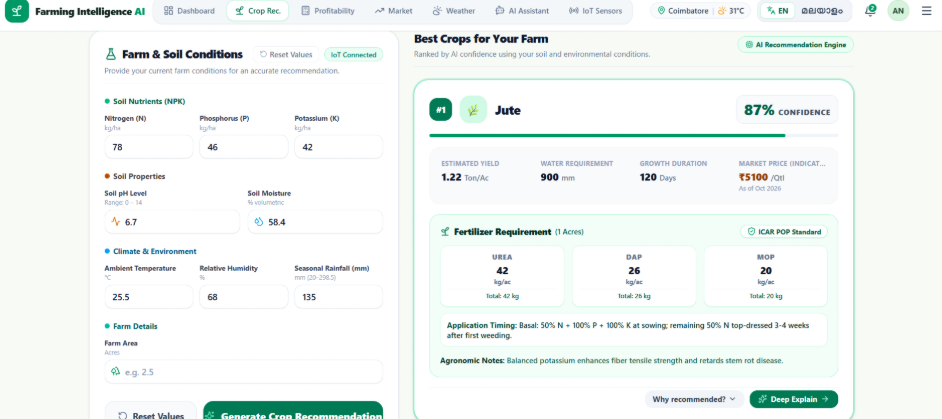
\includegraphics[width=0.8\linewidth]{img/crop_recommendation_results.png}
    \caption{Crop Recommendation Input Parameters and Results}
    \label{fig:crop_recommendation_results}
\end{figure}

\begin{figure}[htbp]
    \centering
    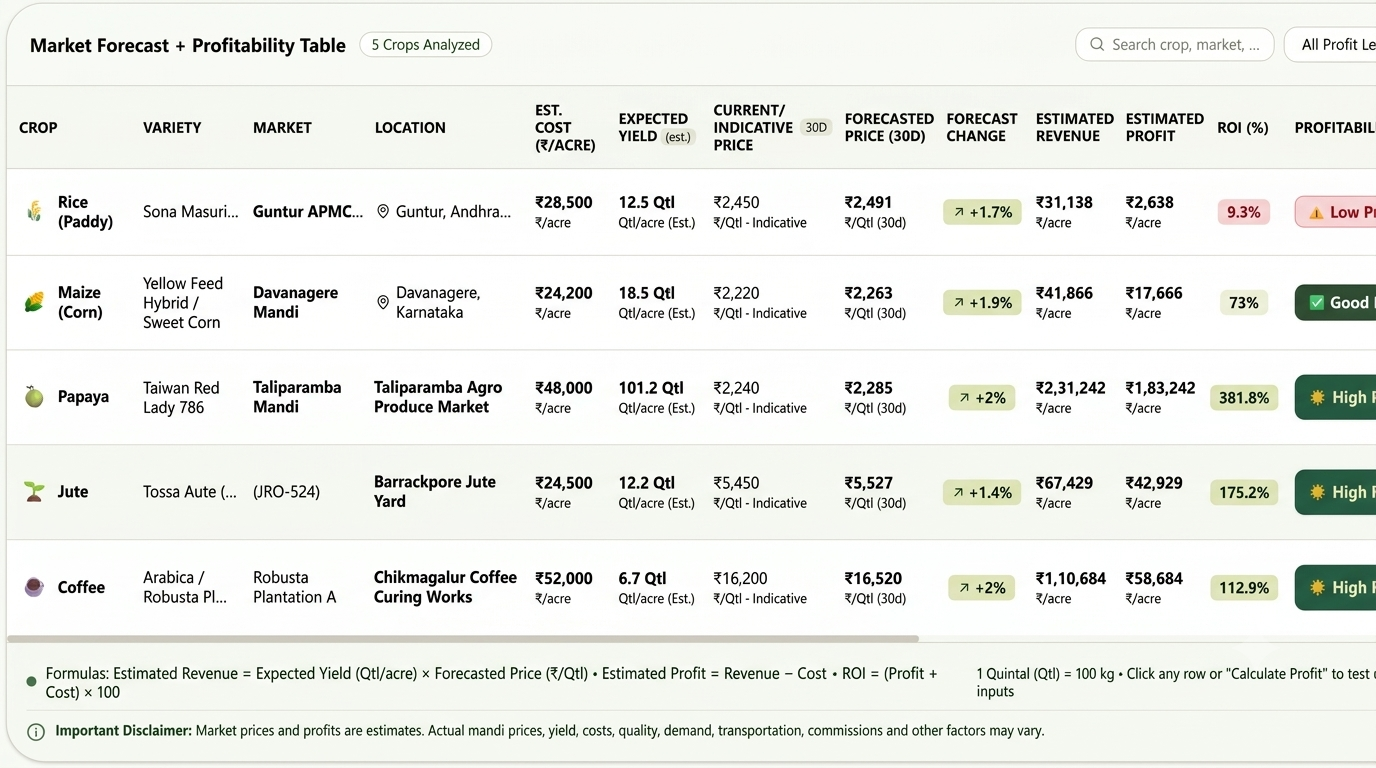
\includegraphics[width=\linewidth]{img/pf.png}
    \caption{Market Forecast and Profitability Table showing crop cost, yield, price predictions, and profitability level.}
    \label{fig:market_profitability_table}
\end{figure}

\begin{figure}[htbp]
    \centering
    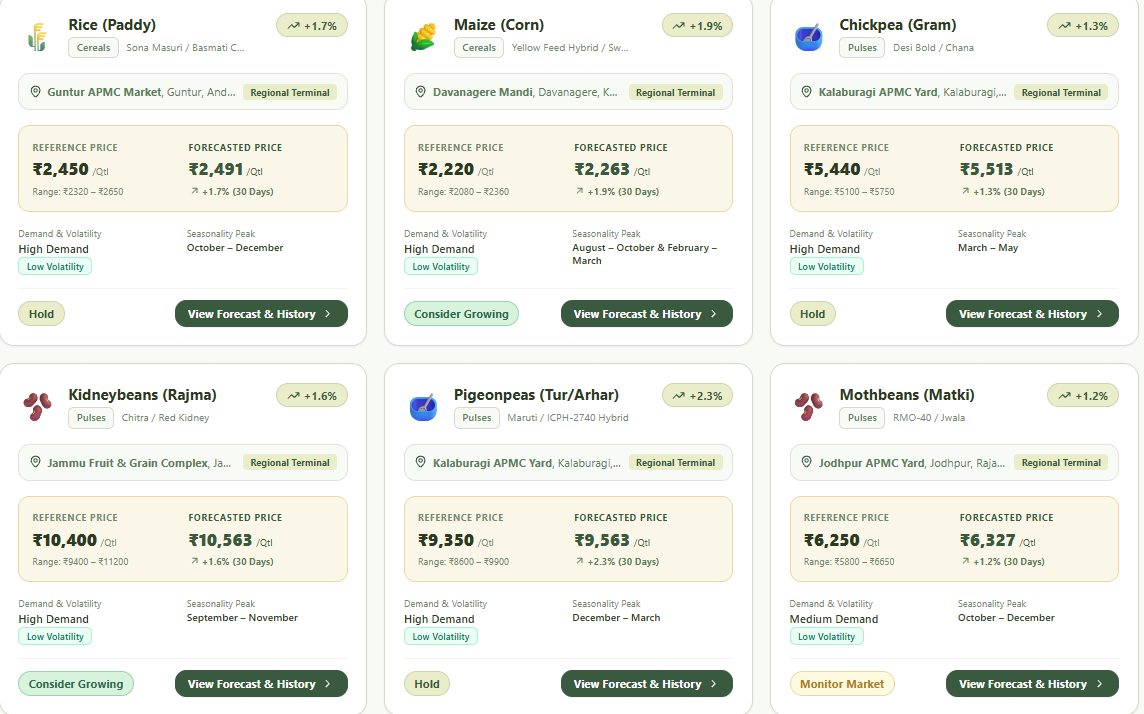
\includegraphics[width=\linewidth]{img/market.png}
    \caption{Market Forecast Cards displaying price trends, demand, and seasonality for various crops.}
    \label{fig:market_forecast_cards}
\end{figure}
\begin{figure}[htbp]
  \centering
  \begin{minipage}[b]{0.8\textwidth}
    \centering
    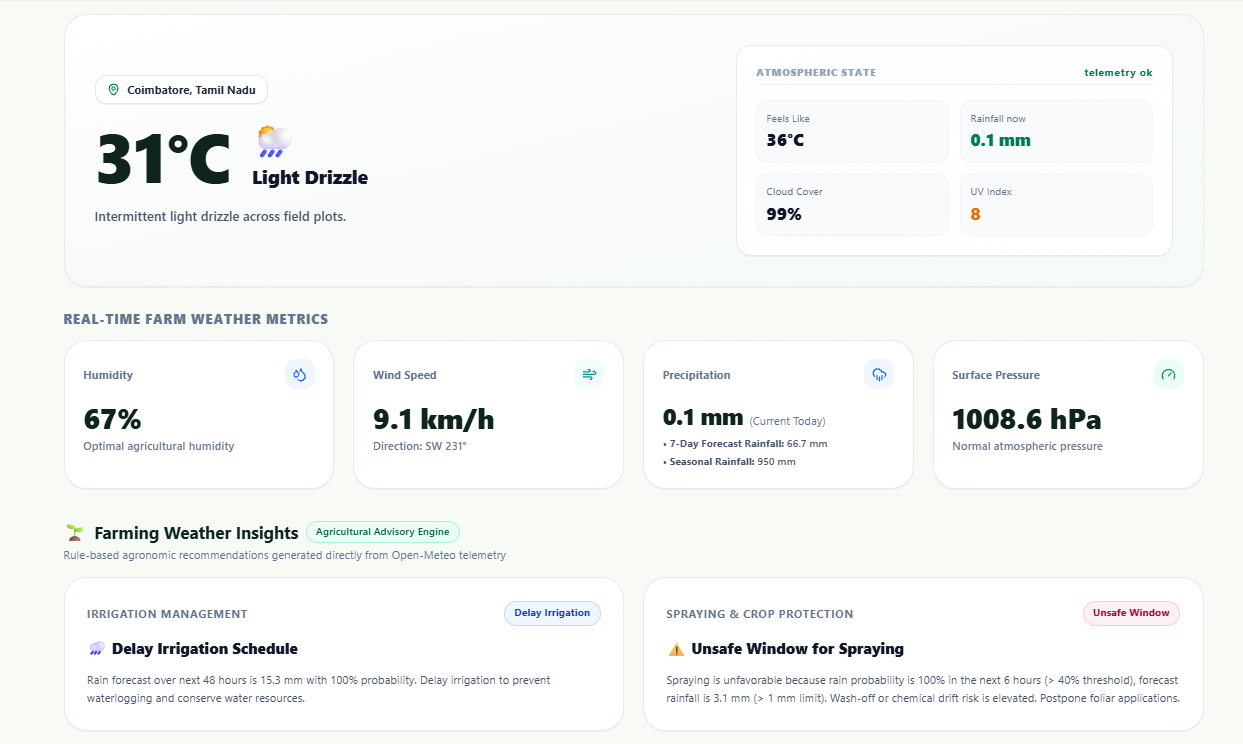
\includegraphics[width=\linewidth]{img/w1.png}
    \caption{Real-Time Farm Weather Metrics}
    \label{fig:real_time_weather}
  \end{minipage}
  \hfill
  \begin{minipage}[b]{0.8\textwidth}
    \centering
    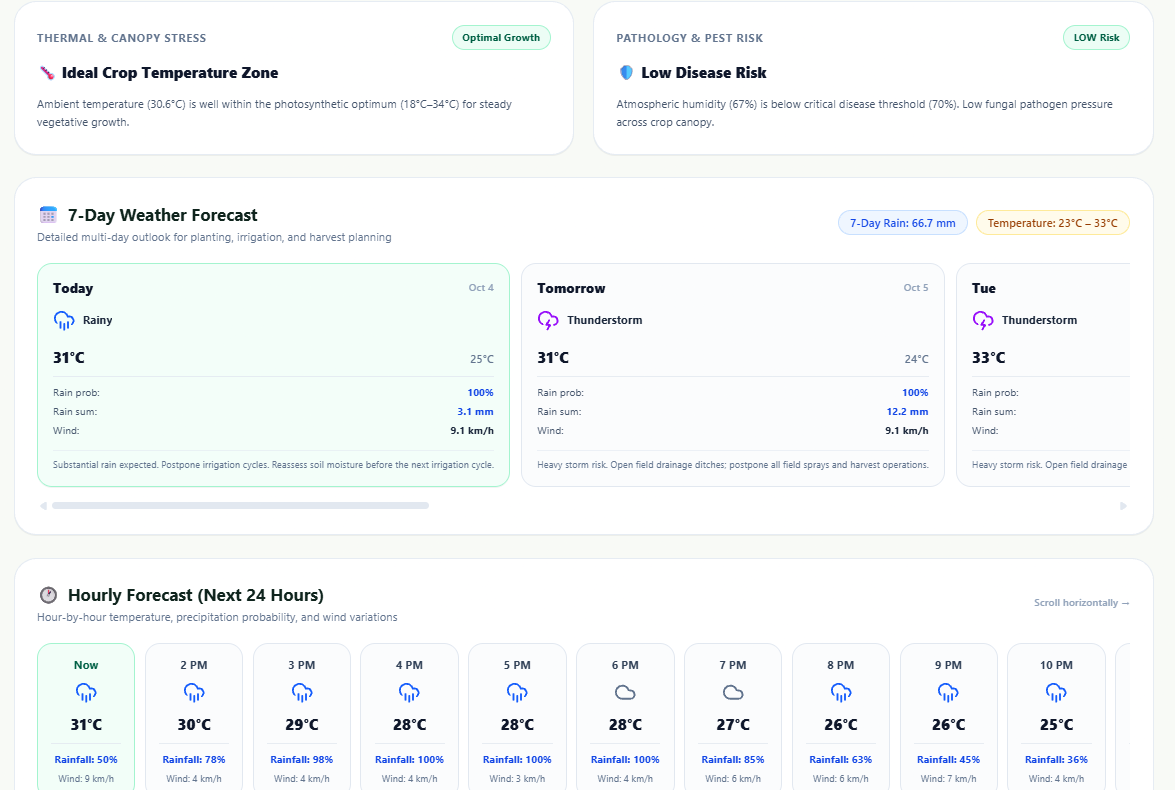
\includegraphics[width=\linewidth]{img/w2.png}
    \caption{7-Day Weather Forecast Details}
    \label{fig:7_day_forecast}
  \end{minipage}
\end{figure}

\begin{figure}[htbp]
    \centering
    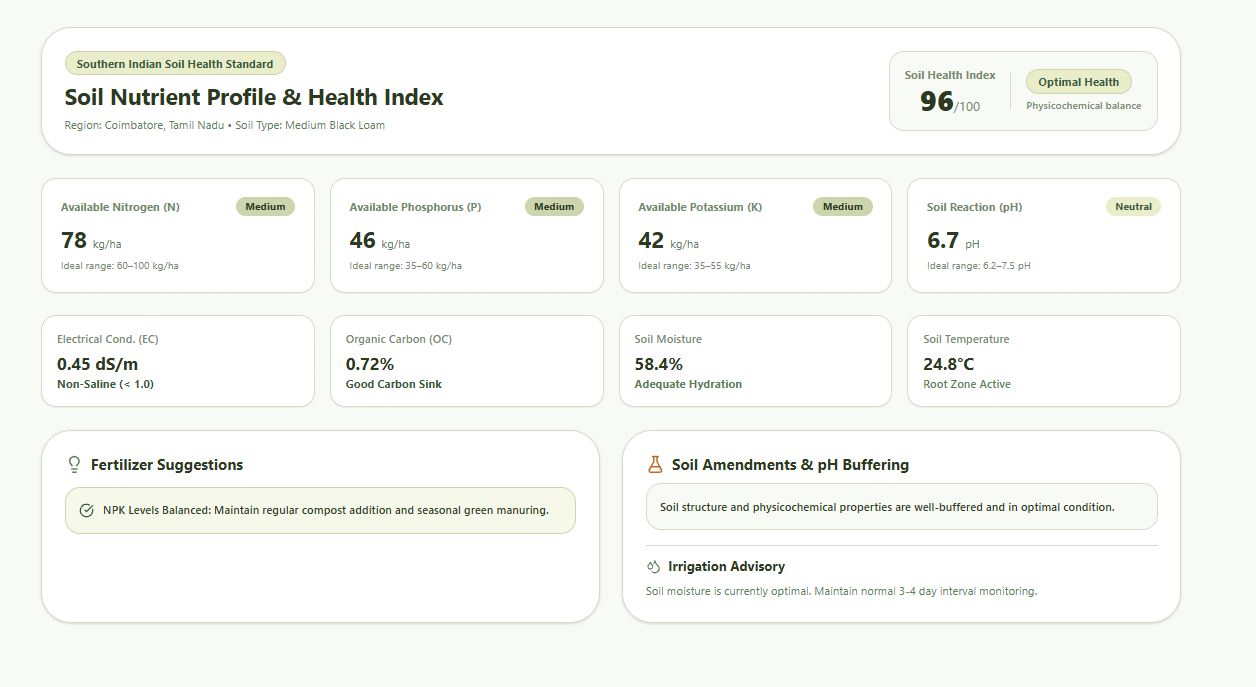
\includegraphics[width=1.0\linewidth]{img/soil_health.png}
    \caption{Soil Nutrient Profile and Health Index Dashboard}
    \label{fig:soil_nutrient_profile}
\end{figure}

\begin{figure}[htbp]
    \centering
    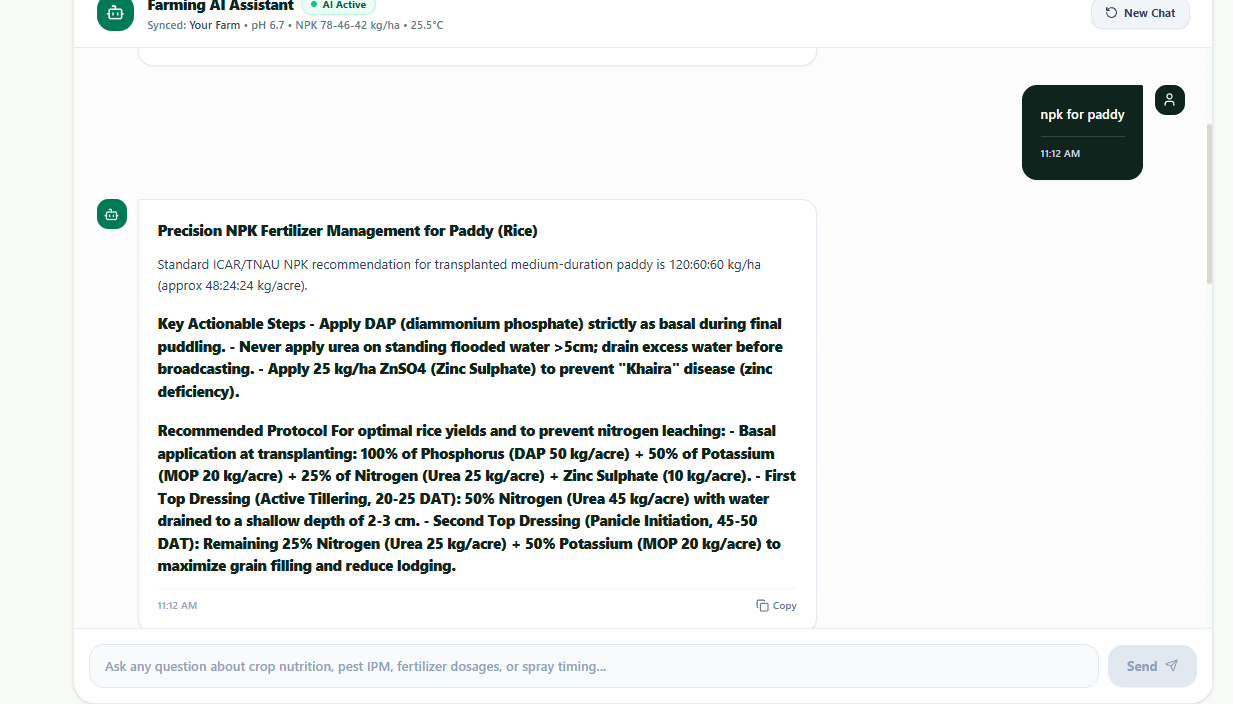
\includegraphics[width=1.0\linewidth]{img/xai.png}
    \caption{Farming AI Assistant Interface showing NPK fertilizer advisory for Paddy.}
    \label{fig:ai_assistant_paddy}
\end{figure}

\begin{figure}[htbp]
    \centering
    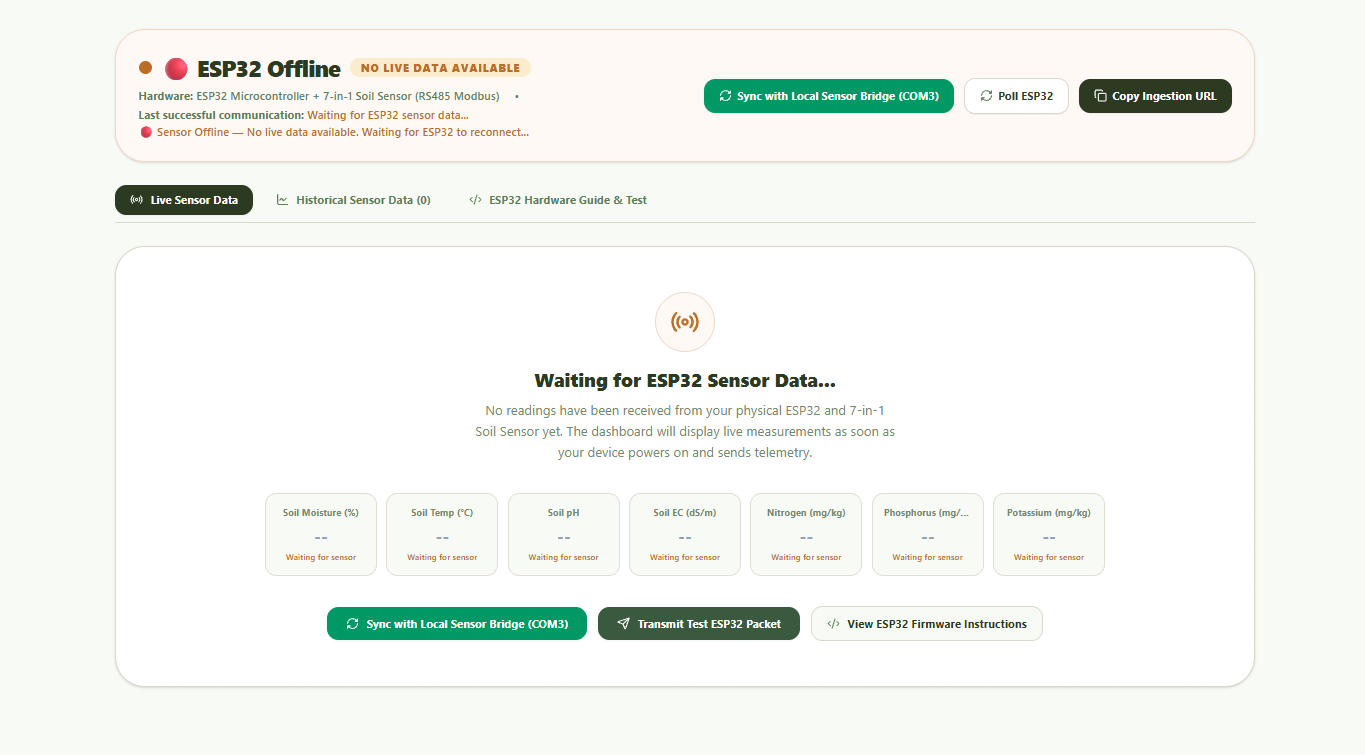
\includegraphics[width=0.8\linewidth]{img/iot.png}
    \caption{IoT Sensor Data Dashboard displaying ESP32 status and telemetry connection controls.}
    \label{fig:esp32_sensor}
\end{figure}
\begin{figure}[htbp]
    \centering
    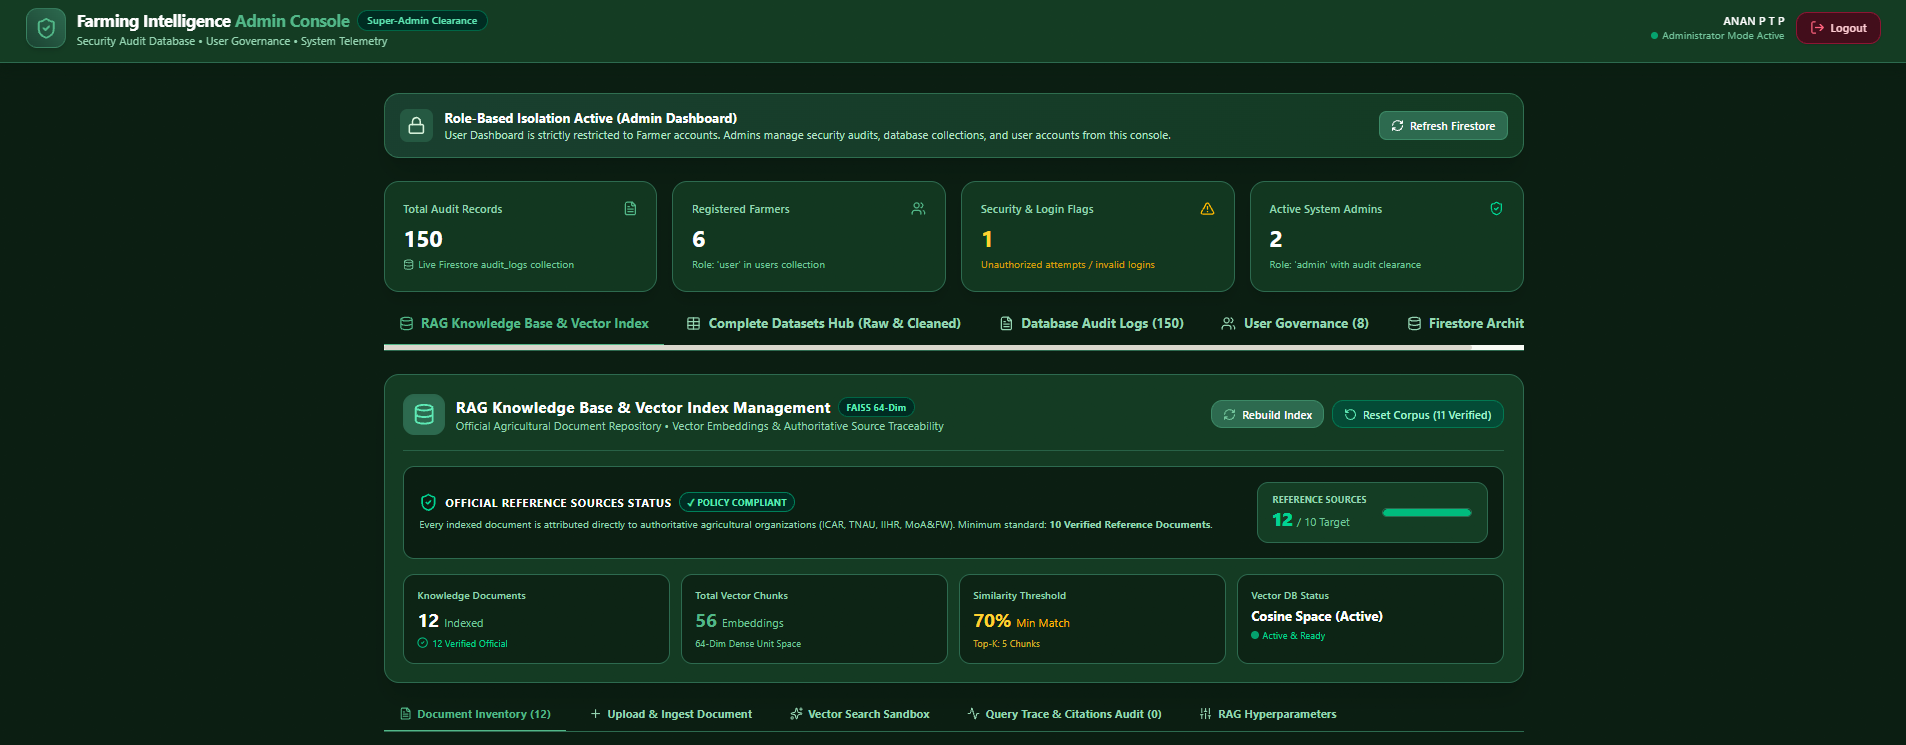
\includegraphics[width=0.8\linewidth]{img/admin1.png}
    \caption{Farming Intelligence Admin Console displaying system telemetry, security audit metrics, and RAG Knowledge Base \& Vector Index management.}
    \label{fig:admin_console_rag}
\end{figure}

\begin{figure}[htbp]
    \centering
    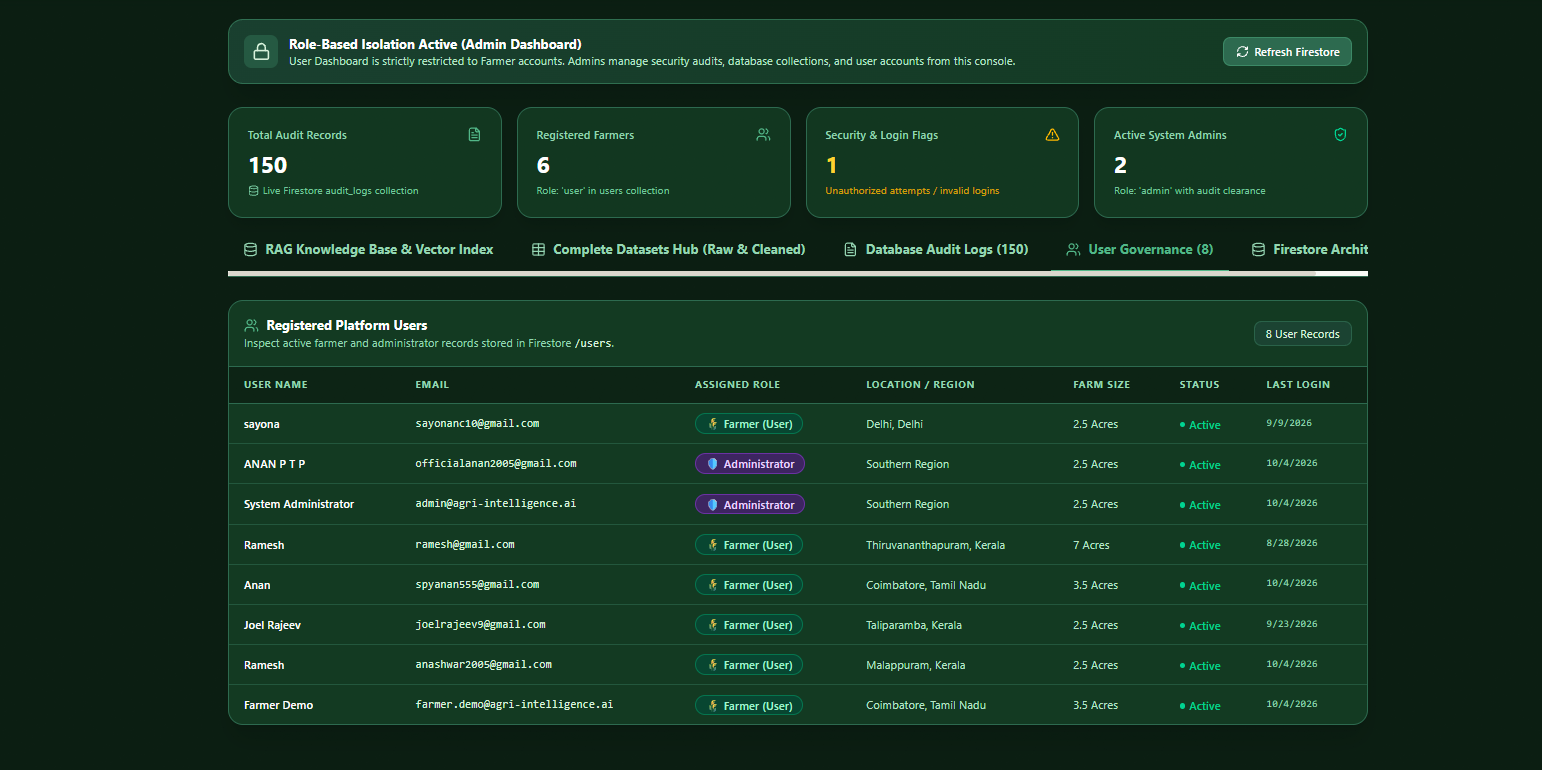
\includegraphics[width=0.8\linewidth]{img/admin2.png}
    \caption{Farming Intelligence Admin Console displaying User Governance and registered platform users.}
    \label{fig:admin_console_user_governance}
\end{figure}

\begin{figure}[htbp]
    \centering
    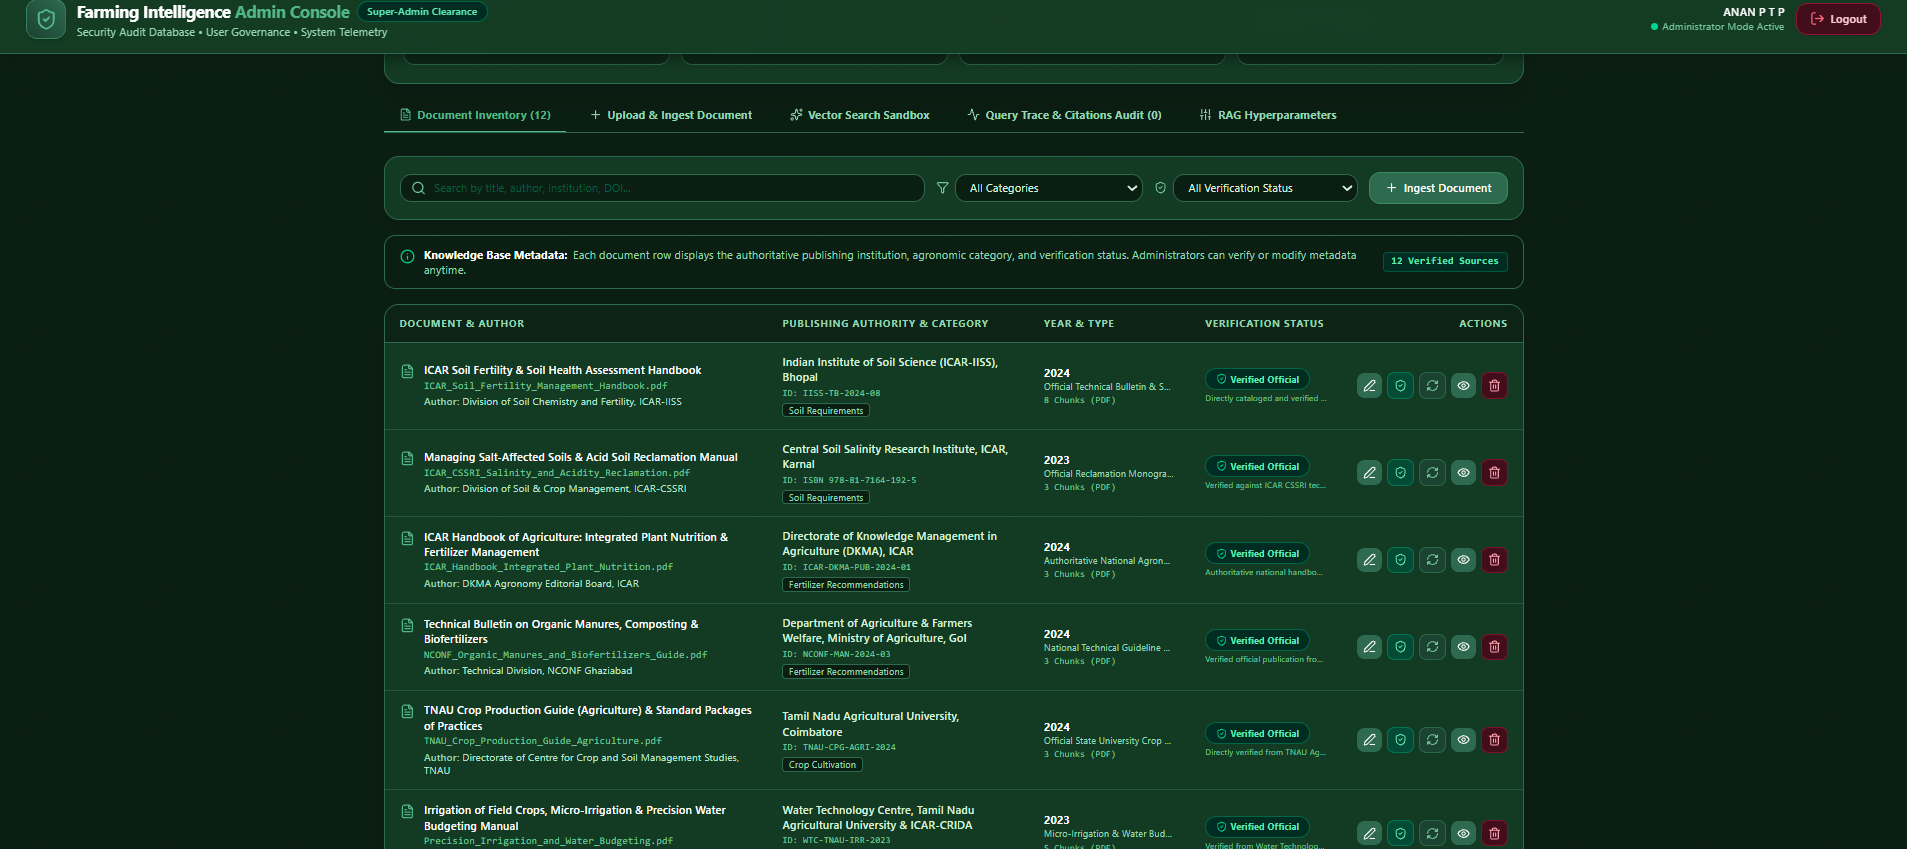
\includegraphics[width=1.0\linewidth]{img/rag.png}
    \caption{Admin Console RAG Knowledge Base Document Inventory showing verified reference sources, publishing authorities, and metadata.}
    \label{fig:admin_console_document_inventory}
\end{figure}

\begin{figure}[htbp]
    \centering
    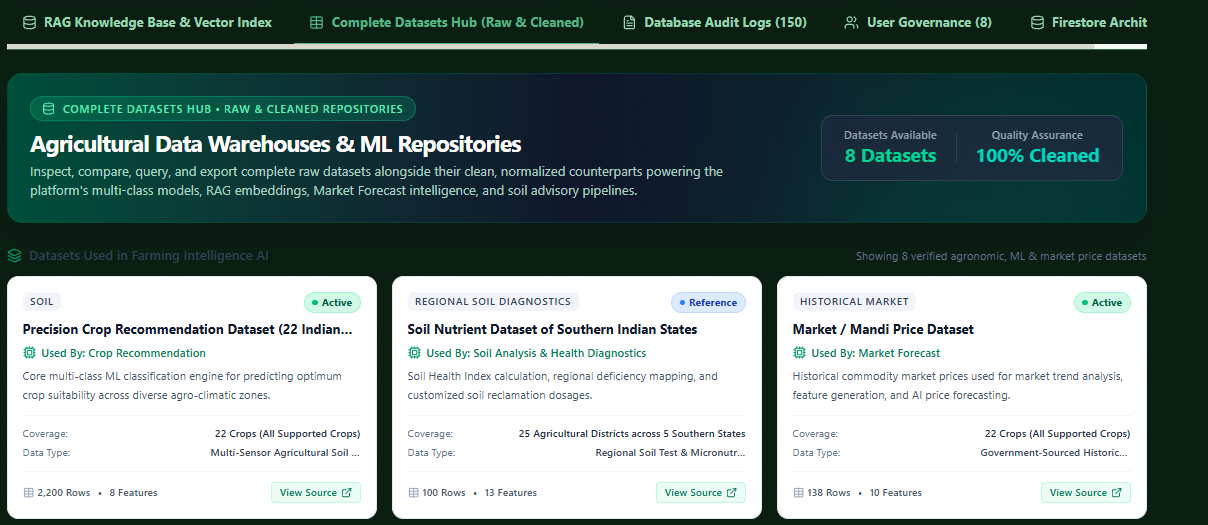
\includegraphics[width=1.1\linewidth]{img/datasets.png}
    \caption{Farming Intelligence Admin Console Datasets Hub displaying active agricultural data repositories and machine learning datasets.}
    \label{fig:admin_console_datasets_hub}
\end{figure}